\chapter{\IfLanguageName{dutch}{Stand van zaken}{State of the art}}%
\label{ch:stand-van-zaken}

% Tip: Begin elk hoofdstuk met een paragraaf inleiding die beschrijft hoe
% dit hoofdstuk past binnen het geheel van de bachelorproef. Geef in het
% bijzonder aan wat de link is met het vorige en volgende hoofdstuk.

% Pas na deze inleidende paragraaf komt de eerste sectiehoofding.

% Dit hoofdstuk bevat je literatuurstudie. De inhoud gaat verder op de inleiding, maar zal het onderwerp van de bachelorproef *diepgaand* uitspitten. De bedoeling is dat de lezer na lezing van dit hoofdstuk helemaal op de hoogte is van de huidige stand van zaken (state-of-the-art) in het onderzoeksdomein. Iemand die niet vertrouwd is met het onderwerp, weet nu voldoende om de rest van het verhaal te kunnen volgen, zonder dat die er nog andere informatie moet over opzoeken \autocite{Pollefliet2011}.

% Je verwijst bij elke bewering die je doet, vakterm die je introduceert, enz.\ naar je bronnen. In \LaTeX{} kan dat met het commando \texttt{$\backslash${textcite\{\}}} of \texttt{$\backslash${autocite\{\}}}. Als argument van het commando geef je de ``sleutel'' van een ``record'' in een bibliografische databank in het Bib\LaTeX{}-formaat (een tekstbestand). Als je expliciet naar de auteur verwijst in de zin (narratieve referentie), gebruik je \texttt{$\backslash${}textcite\{\}}. Soms is de auteursnaam niet expliciet een onderdeel van de zin, dan gebruik je \texttt{$\backslash${}autocite\{\}} (referentie tussen haakjes). Dit gebruik je bv.~bij een citaat, of om in het bijschrift van een overgenomen afbeelding, broncode, tabel, enz. te verwijzen naar de bron. In de volgende paragraaf een voorbeeld van elk.

% \textcite{Knuth1998} schreef een van de standaardwerken over sorteer- en zoekalgoritmen. Experten zijn het erover eens dat cloud computing een interessante opportuniteit vormen, zowel voor gebruikers als voor dienstverleners op vlak van informatietechnologie~\autocite{Creeger2009}.

% Let er ook op: het \texttt{cite}-commando voor de punt, dus binnen de zin. Je verwijst meteen naar een bron in de eerste zin die erop gebaseerd is, dus niet pas op het einde van een paragraaf.


% \begin{figure}
%   \centering
%   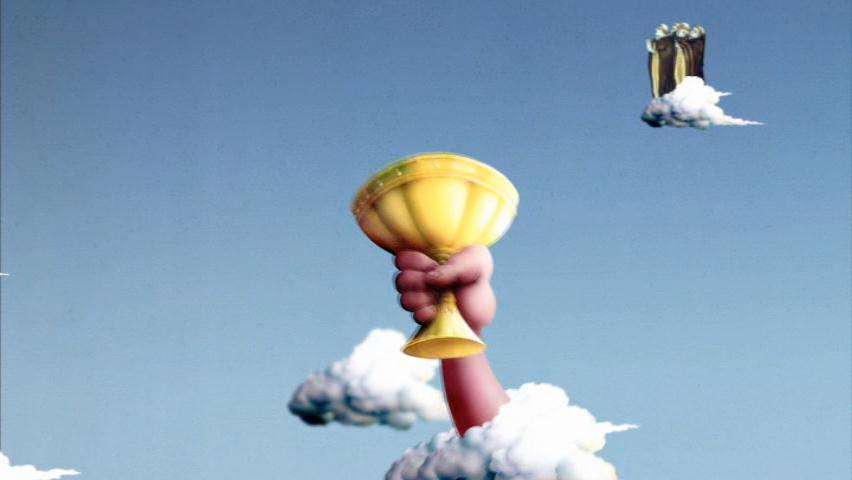
\includegraphics[width=0.8\textwidth]{grail.jpg}
%   \caption[Voorbeeld figuur.]{\label{fig:grail}Voorbeeld van invoegen van een figuur. Zorg altijd voor een uitgebreid bijschrift dat de figuur volledig beschrijft zonder in de tekst te moeten gaan zoeken. Vergeet ook je bronvermelding niet!}
% \end{figure}

% \begin{listing}
%   \begin{minted}{python}
%     import pandas as pd
%     import seaborn as sns

%     penguins = sns.load_dataset('penguins')
%     sns.relplot(data=penguins, x="flipper_length_mm", y="bill_length_mm", hue="species")
%   \end{minted}
%   \caption[Voorbeeld codefragment]{Voorbeeld van het invoegen van een codefragment.}
% \end{listing}

% \begin{table}
%   \centering
%   \begin{tabular}{lcr}
%     \toprule
%     \textbf{Kolom 1} & \textbf{Kolom 2} & \textbf{Kolom 3} \\
%     $\alpha$         & $\beta$          & $\gamma$         \\
%     \midrule
%     A                & 10.230           & a                \\
%     B                & 45.678           & b                \\
%     C                & 99.987           & c                \\
%     \bottomrule
%   \end{tabular}
%   \caption[Voorbeeld tabel]{\label{tab:example}Voorbeeld van een tabel.}
% \end{table}

Geautomatiseerde dataverzameling en -analyse spelen een steeds grotere rol in de professionele sportwereld, waar nauwkeurige statistieken noodzakelijk zijn voor prestatieverbetering en strategische besluitvorming. In de sport, in het bijzonder in volleybal, zorgt automatisering van statistiekenverzameling ervoor dat spelers en coaches beter inzicht krijgen in prestaties, waardoor training en wedstrijdvoorbereiding doelgerichter kunnen worden aangepakt.

\section{Belang van statistieken in de sportwereld}
Vooral technologieën zoals AI, computer vision en machine learning bieden nieuwe mogelijkheden om spelmomenten en spelersbewegingen nauwkeurig vast te leggen en te analyseren. De spelers- en matchstatistieken \autocite{Wahyuti2023} zijn van uiterst belang. Ze bieden niet alleen inzichten in de puntenregistratie van het team, maar ook in de tactische en technische aspecten van het spel. Volgens de studie is het belangrijk om een uitgebreid digitaal puntenregistratie bij te houden. Dit om fouten en verlies van gegevens te minimaliseren. Dit komt echter vaak voor bij handmatige invoer. Uit onderzoek \autocite{Harabagiu2023} blijkt dat door gebruik van de statistische software Data Volley de efficiënte van een team met 6\% stijgt. De software identificeert de tekortkomingen en hierdoor kunnen individuele trainingsprogramma's opgesteld worden voor elke speler. Volgens \textcite{Ruiye2024} zijn de nauwkeurigheid en efficiëntie van de videoanalyse zeer belangrijk. Een innovatief videoanalysemodel gebaseerd op Bi-directional Long Short-Term Memory (BiLSTM) en aandachtsmechanismen behaalt een herkenningsnauwkeurigheid van meer dan 90\%.

Natuurlijk zijn er andere invloeden op de statistieken dan alleen de spelersprestaties \autocite{LopezSerrano2022}. Zo spelen volgens verschillende coaches het niveau van de tegenstander, het moment in een set, het scoreverschil, resultaat van de vorige set en het de competitieve druk een zeer grote in de analyse. Trainers pleiten ervoor dat er een geïntegreerde benadering is voor deze variabelen. Hierdoor wordt rekening gehouden met de specifieke omstandigheden van elke wedstrijd. Deze gegevens mogen niet geïsoleerd worden bekeken, maar juist in samenhang geanalyseerd. Bij verder onderzoek is het van essentieel belang dat coaches worden betrokken bij de ontwikkeling hiervan.

\section{Toepassing van kunstmatige intelligentie en data-analyse}
\textcite{Fadl2020} benadrukt het belang van moderne technologieën in de sport en hoe deze kunnen bijdragen aan het verbeteren van coachingsmethoden.

Om dit te bereiken, werd een beoordelingssysteem ontwikkeld waarmee coaches de bewegingsanalyse van spelers efficiënter kunnen uitvoeren. Dit systeem werd geëvalueerd door 200 ervaren volleybalcoaches en bleek binnen een korte tijdspanne van maximaal 15 minuten bruikbare inzichten te bieden. De methode omvatte verschillende analysecomponenten, zoals technische observatie, prestatiediagnose en trainingsinterventies, om coaches te helpen bij het plannen en optimaliseren van trainingssessies.
Uit de resultaten bleek dat AI-gestuurde bewegingsanalyse een effectief hulpmiddel is om trainers te ondersteunen bij het kwantificeren van prestaties en het identificeren van verbeterpunten.
Deze bevindingen onderstrepen hoe technologische vooruitgang kan bijdragen aan een betere trainingservaring, door coaches te voorzien van nauwkeurige en snelle analytische tools voor het verbeteren van de prestaties van hun spelers.

\textcite{Huang2023} ontwikkelen een AI-gestuurd model voor de detectie en herkenning van overtredingen in volleybal, ter vervanging van subjectieve scheidsrechtersoordelen. Het model maakt gebruik van videoverbeteringstechnologie en een combinatie van algoritmen, waaronder de wavelet-transformatie, de drie-frame verschilmethode en achtergrondsubtractie, om bewegende objecten te identificeren. De wavelet-transformatie is een techniek die signalen in verschillende frequenties analyseert en zowel tijd- als frequentiedomein-informatie biedt, wat helpt bij het extraheren van belangrijke kenmerken van bewegende objecten, zoals spelers en de bal. De drie-frame verschilmethode vergelijkt opeenvolgende frames in een video om veranderingen te detecteren, wat effectief helpt bij het identificeren van de beweging van objecten, zoals de bal en de spelers. Daarnaast wordt achtergrondsubtractie toegepast, waarbij het verschil tussen de huidige beeldinhoud en een vooraf gedefinieerd achtergrondmodel wordt berekend, zodat alleen de bewegende objecten ten opzichte van de achtergrond worden geïdentificeerd.
De verbeterde CamShift-trackingmethode, ondersteund door een Kalman-filter, optimaliseert de tracking van spelers door dynamisch de grootte en positie van zoekgebieden aan te passen op basis van de kleurverdeling van de objecten, wat zorgt voor nauwkeurige objectvolging. Bovendien wordt een Hidden Markov Model (HMM) ingezet voor de classificatie van overtredingen. Het HMM is een statistisch model dat de toestand van het spel op basis van sequentiële data analyseert en de waarschijnlijkheid van een overtreding voorspelt op basis van eerdere gedragingen en de huidige staat van het spel.
Uit experimentele resultaten blijkt dat het model een hoge herkenningsnauwkeurigheid heeft (99,76\%) en een gemiddelde foutmarge van 0,003. Hiermee biedt het een objectieve en betrouwbare methode voor scheidsrechtersbeslissingen, wat bijdraagt aan de eerlijkheid en nauwkeurigheid van arbitrage in volleybal. Dit onderzoek benadrukt de potentie van AI in sportanalyse en opent mogelijkheden voor bredere toepassingen in andere sporten.

\textcite{Liu2021} introduceren een innovatief model voor sportdata-visualisatie, het Video-based Effective Visualization Framework (VEVF). Dit model combineert kunstmatige intelligentie (AI) en big data-analyse om sportvideo's te classificeren en te analyseren, met als doel de prestaties van atleten te verbeteren en coaches en analisten van waardevolle inzichten te voorzien.
Het belang van data-visualisatie in de sportwereld wordt nogmaals benadrukt, vooral in het tijdperk van big data. Sportdata, zoals atleetprestaties, trainingsstatistieken en gezondheidsgegevens, kunnen worden gebruikt om betere spelstrategieën te ontwikkelen, blessures te verminderen en de prestaties van atleten te verbeteren. Het VEVF-model maakt gebruik van draagbare apparaten om real-time bewegingsdata van atleten te verzamelen en deze te visualiseren in een 3D-virtuele omgeving. Dit stelt coaches in staat om de prestaties van atleten beter te monitoren en toekomstige bewegingen te voorspellen.

\section{Gebruik van sensors en camera's voor dataverzameling}
Uit onderzoek van Xu \textcite{Sun2021} blijkt dat door de vooruitgang in elektronische en sensortechnologieën het mogelijk is geworden om menselijke bewegingen en spelmomenten nauwkeurig vast te leggen. In de sportwereld zijn sensoren en camera's steeds vaker te vinden op en naast het veld. Deze technologieën maken het mogelijk om realtime data te verzamelen over spelersposities, balbewegingen en spelsituaties door middel van sensoren aan de gewrichten van spelers te bevestigen. Door deze data te analyseren met behulp van AI-algoritmen kunnen coaches en analisten waardevolle inzichten verkrijgen in de prestaties en strategieën.

Het onderzoek van \textcite{Salim2024} richt zich op het optimaliseren van volleybaltraining door middle van geavanceerde sensortechnologie en data-analyse. Er wordt een innovatief platform gepresenteert dat gebruikmaakt van een drukgevoelige vloer en machine learning om zowel atleten als coaches te ondersteunen. Het systeem kan automatisch verschillende volleybalacties herkennen. Artificiële intelligentie gaat deze acties detecteren en direct feedback geven aan de spelers. Daarnaast kan het ook automatisch belangrijke speelmomenten markeren.
Naast analyse biedt het systeem ook interactieve leeromgevingen, waarbij trainingen dynamisch worden aangepast op basis van de waargenomen bewegingen van spelers. Dit wordt mogelijk gemaakt door een combinatie van machine learning-modellen, waaronder convolutionele neurale netwerken (CNN) en actieve datarepresentatie (ADR). Convolutionele neurale netwerken vormen een klasse van diepe neurale netwerken die bijzonder geschikt zijn voor de verwerking en analyse van visuele gegevens. Ze bootsen de werking van het menselijk visuele systeem na door gebruik te maken van convolutielagen, waarbij kleine filters of kernels over een afbeelding schuiven om patronen en kenmerken zoals randen, vormen en texturen te detecteren. Dit maakt CNN's zeer effectief voor taken zoals beeldherkenning, objectdetectie en actieclassificatie, wat cruciaal is in interactieve leeromgevingen waarbij spelersbewegingen worden geanalyseerd en gebruikt om trainingen dynamisch aan te passen. Deze technologieën behaalden een nauwkeurigheid tot 78,71\% bij het herkennen van acties.
Deze technologie heeft wel nog verdere verbeteringen nodig vooraleer het in de praktijk kan toegepast worden, maar het toont wel aan dat de manier waarop volleybaltrainingen vorm krijgen fundamenteel kunnen veranderen.

\textcite{Liang2023} concludeerden dat traditionele videoanalysemethode vaak te beperkt is voor de variabele omstandigheden zoals verlichting en achtergrond tijdens het spel. Skeletdata biedt hier een oplossing voor door de bewegingen van spelers te vereenvoudigen tot een netwerk van verbonden gewrichten. De complexiteit van de visuele gegevens vermindert hierdoor. De methode zou nog een extra assistentie kunnen bieden aan de coaches en spelers.

\section{Gebruik van machine learning voor analyse van volleybaldata}
De integratie van machine learning en digitale informatietechnologie in volleybal biedt nieuwe mogelijkheden voor prestatieverbetering en spelanalyse.

\textcite{Musa2021} onderzoeken welke factoren bijdragen aan het identificeren van getalenteerde volleybalspelers. Hierbij werd gekeken naar zowel fysieke kenmerken, zoals lengte, gewicht en leeftijd, als psychologische aspecten, waaronder mentale weerbaarheid en voorbereiding op wedstrijden. Door middel van machine learning werden spelers ingedeeld in twee prestatiecategorieën: hoogpresterend (HVP) en laagpresterend (LVP).
Uit de resultaten bleek dat gewicht, leeftijd en psychologische vaardigheden significante verschillen vertoonden tussen de twee groepen, terwijl lengte geen doorslaggevende factor was. Hoogpresterende spelers blonken vooral uit in mentale strategieën zoals zelfspraak, visualisatie en emotieregulatie, wat een belangrijke rol bleek te spelen bij succes op het veld.
Deze studie benadrukt het belang van zowel fysieke als mentale factoren bij het selecteren van talentvolle volleybalspelers. Daarnaast laat het zien hoe machine learning kan worden ingezet als hulpmiddel voor coaches bij het scouten en samenstellen van teams.

Het onderzoek van \textcite{Dai2021} richt zich op het gebruik van machine learning voor de analyse van volleybaldata. Het doel is om spelers en coaches meer inzicht te geven in de technische uitvoering van bewegingen, met name de smash zoals afgebeeld in figuur \ref{fig:spike} en de bijbehorende spieractiviteit. In het experiment werden twaalf volleybalspelers onderverdeeld in twee groepen: één groep gebruikte een preswing-techniek met beide armen (type A), terwijl de andere groep deze techniek niet toepaste (type B).
Door middel van kinematische, dynamische en elektromyografische analyses werden de verschillende fasen van de smash bestudeerd, van de aanloop en afzet tot het moment van raken. De resultaten toonden aan dat type A-spelers over het algemeen een betere balans hadden in spieractiviteit tussen beide zijden van het lichaam. Bij type B-spelers werd daarentegen een grotere afhankelijkheid van de beenspieren vastgesteld, wat suggereert dat zij compenseren voor het ontbreken van een preswing-beweging met de armen.
Daarnaast bleek dat de kracht die tijdens de sprong werd gegenereerd, bij type A hoger was dan bij type B, wat duidt op een efficiëntere energieoverdracht. Ook was er een verschil in de bijdrage van de rompspieren, waarbij de rechte buikspier bij type A een evenwichtige rol speelde, terwijl deze bij type B een dominante functie had.

\begin{figure}
  \centering
  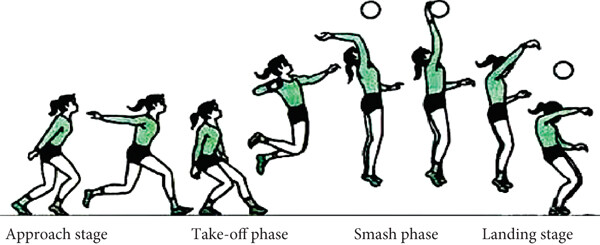
\includegraphics[width=0.8\textwidth]{img/spike.jpg}
  \caption{\label{fig:spike}Een reeks actiediagrammen van volleybal-spikes.}
  \autocite{Dai2021}
\end{figure}

Machine learning kan ook worden ingezet om blessures bij professionele volleyballers te monitoren en te voorspellen, volgens \textcite{Leeuw2021}. Door dagelijks gegevens te verzamelen over trainingsbelasting, sprongbelasting en welzijnsindicatoren, probeerden de onderzoekers inzicht te krijgen in het ontstaan en de ontwikkeling van overbelastingsblessures.
Voor dit onderzoek werden veertien topspelers gedurende 24 weken gevolgd. Ze vulden dagelijks vragenlijsten in over hun fysieke toestand en blessures, terwijl hun fysieke activiteiten en sprongbelasting werden geregistreerd via draagbare sensoren. De gegevens werden geanalyseerd met de machine learning-techniek Subgroup Discovery, waarmee verbanden tussen trainingsbelasting, welzijn en blessurerisico per individuele speler werden geïdentificeerd.
Uit de resultaten bleek dat verhoogde sprongbelasting een belangrijke voorspeller was van overbelastingsblessures, vooral aan de knieën. Daarnaast verschilden de risicofactoren per speler, wat het belang van een gepersonaliseerde aanpak onderstreept. Door patronen te herkennen in trainingsbelasting en blessureklachten, konden de onderzoekers gepersonaliseerd advies formuleren om blessures te helpen voorkomen.

\textcite{Yu2022} verkennen hoe kunstmatige neurale netwerken en genetische algoritmen kunnen bijdragen aan een betere beoordeling van serveer-, landings- en blokkeeracties. Door deze technologieën toe te passen, wordt niet alleen de reactietijd van spelers verbeterd, maar neemt ook de nauwkeurigheid van beslissingen toe, wat essentieel is voor training en blessurepreventie.
Verder worden clustering, regressieanalyse en informatieverwerking gebruikt om patronen in spelprestaties te identificeren en te voorspellen. De bevindingen tonen aan dat spelers met een hoger vaardigheidsniveau efficiënter tactische informatie verwerken en sneller reageren op speelsituaties. Dit onderzoek onderstreept de potentie van AI-gebaseerde technologieën in de sportwetenschap en biedt waardevolle inzichten voor coaching en prestatieanalyse.

\section{Bestaande AI-systemen voor sportstatistieken}
Er zijn verschillende AI-systemen beschikbaar die kunnen worden ingezet voor het verzamelen en analyseren van sportstatistieken. In tabel \ref{tab:tools} worden ze vergeleken met DataVolley, de tool die momenteel wordt gebruikt.

\begin{table}
  \centering
  \begin{tabular}{lcr}
    \toprule
    \textbf{Tool} & \textbf{Real-time} & \textbf{Video-input}\\
    \midrule
    DataVolley & Nee & Handmatige invoer \\
    Balltime AI & Ja & Opgenomen of live \\
    Hudl Volleyball & Ja & Opgenomen of live \\
    Volleymetrics & Nee & Opgenomen \\
    SportsVisio & Ja & Opgenomen of live \\
    Spiideo & Ja & Opgenomen of live \\
    Veo Camera & Ja & Opgenomen \\
    \bottomrule
  \end{tabular}
  \caption[Korte vergelijking bestaande tools]{\label{tab:tools}Korte vergelijking bestaande tools}
\end{table}

Bij de analyse van volleybalwedstrijden en -trainingen worden verschillende tools ingezet om speldata te verzamelen en te verwerken. Deze tools verschillen op twee belangrijke aspecten: real-time verwerking en de wijze van video-input.

Sommige tools bieden real-time analyse, wat betekent dat gegevens direct tijdens de wedstrijd of training verwerkt en geanalyseerd worden. Dit is het geval bij Balltime AI, Hudl Volleyball, SportsVisio, Spiideo en Veo Camera. Andere tools, zoals DataVolley en VolleyMetrics, bieden deze mogelijkheid niet en verwerken gegevens pas achteraf op basis van opgenomen videobeelden of handmatige invoer.

Naast real-time verwerking verschilt ook de manier waarop videobeelden worden gebruikt. DataVolley vereist een handmatige invoer van data, terwijl VolleyMetrics en Veo Camera uitsluitend werken met opgenomen video’s. De andere tools, zoals Balltime AI, Hudl Volleyball, SportsVisio en Spiideo, kunnen zowel opgenomen als live beelden verwerken. Dit maakt deze tools flexibeler in hun toepassing, omdat ze zowel achteraf als tijdens de wedstrijd analyses kunnen leveren.

De keuze voor een bepaalde analysetool hangt af van de specifieke behoeften van de gebruiker. Indien directe feedback gewenst is, zijn tools met real-time verwerking geschikter. Voor diepgaande analyse op basis van bestaande beelden kunnen niet-real-time tools een waardevolle aanvulling zijn.